\section{Rolling Road}
Text

\subsection{BDD}
Text

\begin{figure}[H]
	\centering
	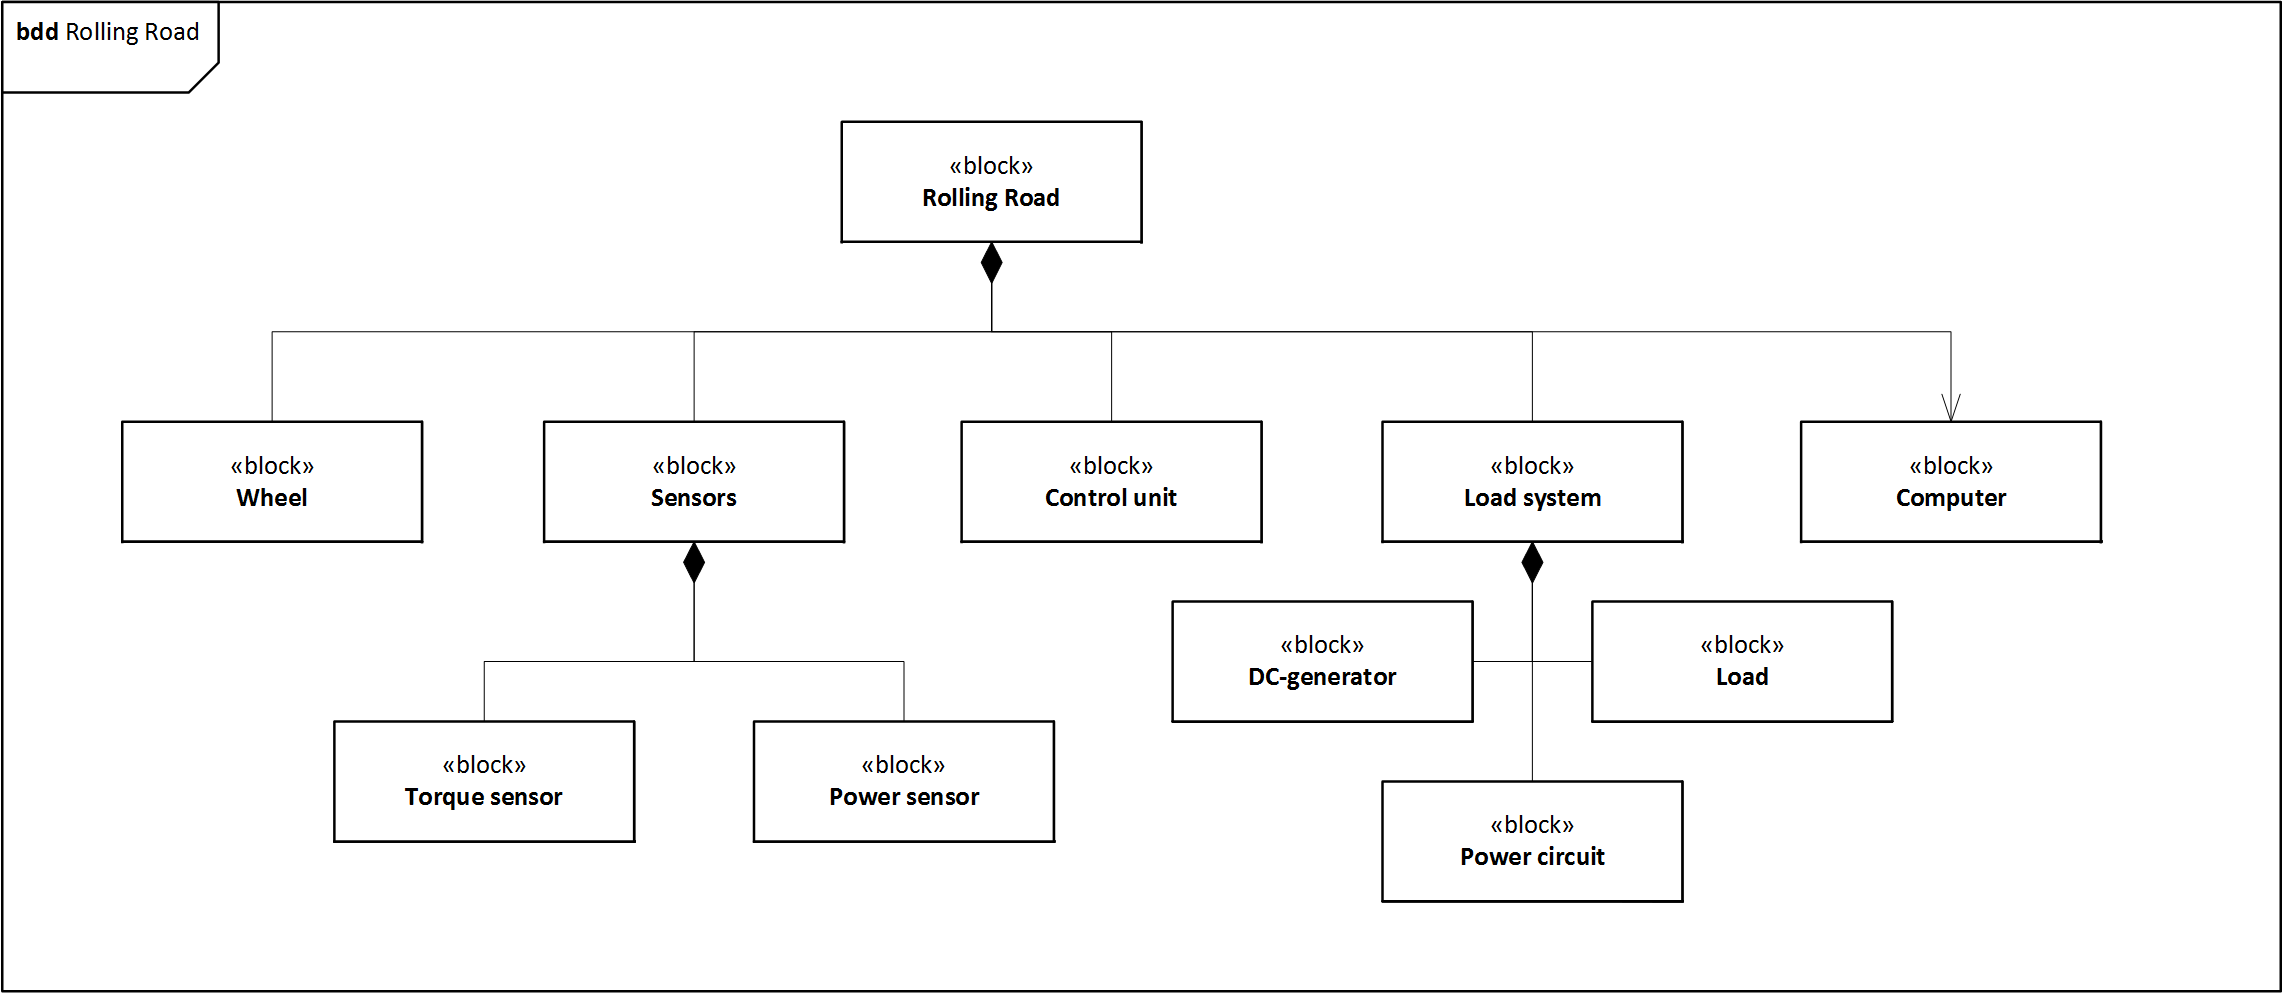
\includegraphics[width=0.9\linewidth]{Architecture/BDD_RollingRoad}
	\caption{BDD for Rolling Road}
	\label{fig:RR_BDD}
\end{figure}

\subsection{IBD}
Text

\begin{figure}[H]
	\centering
	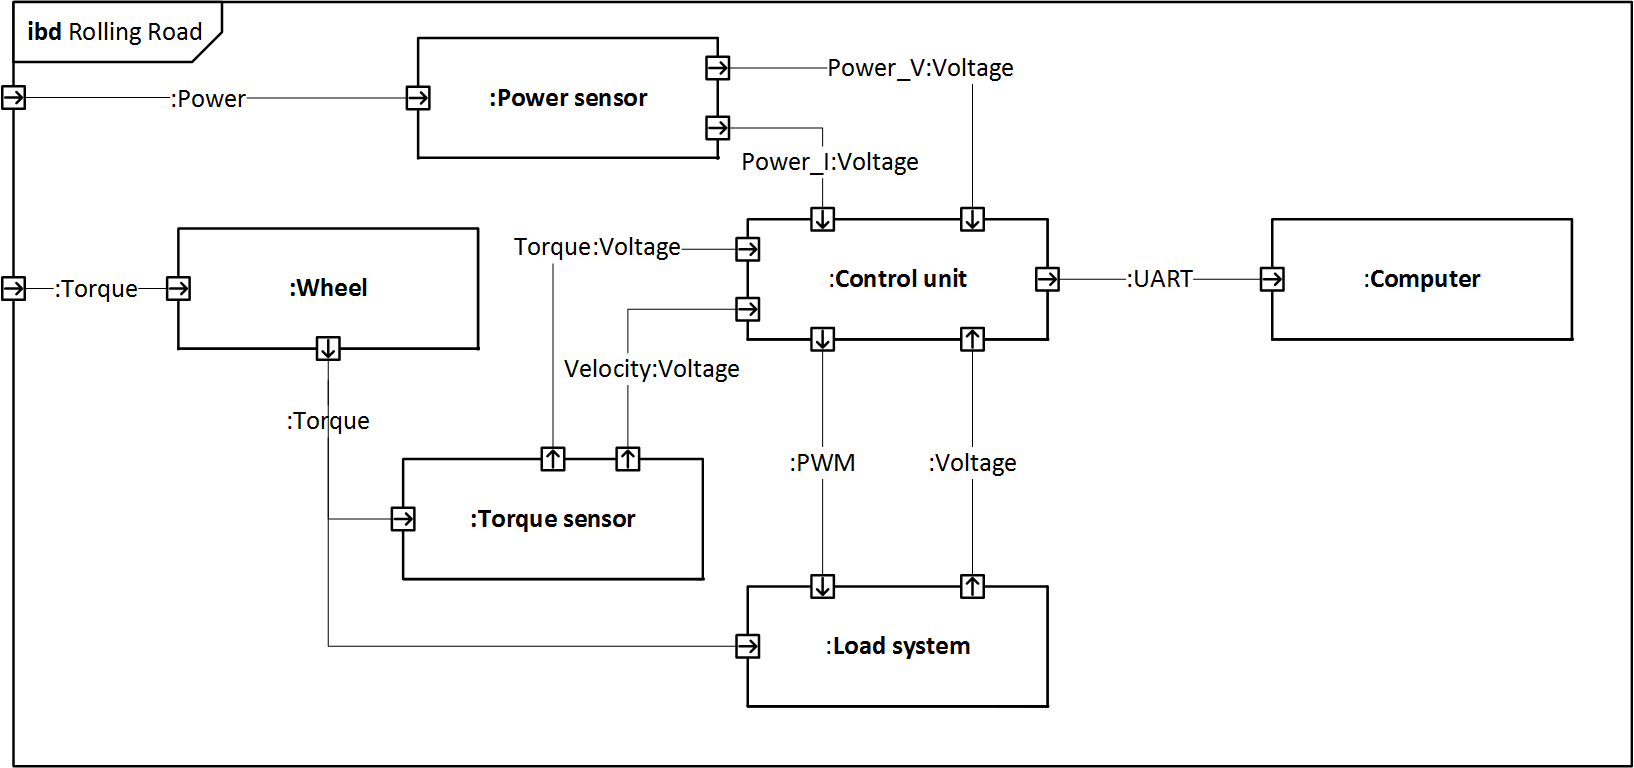
\includegraphics[width=0.9\linewidth]{Architecture/IBD_RollingRoad}
	\caption{IBD for Rolling Road}
	\label{fig:RR_IBD}
\end{figure}

\subsection{Protocol description}
The signals and protocols used to communicate between the blocks are specified in this section.

\textbf{Block :Power sensor}\\
The Power sensor receives power from the external power source (battery). Signals representing the voltage and current emit from the Power sensor as voltage 0-5V.\\
Block interface description:

\begin{itemize}
	\item \textbf{:power}\\
		Direction: [External power source] $\rightarrow$ [Power sensor]\\
		Description: The power received from the external power source.
	\item \textbf{Power\_V :power}\\
		Direction: [Power sensor] $\rightarrow$ [Control unit]\\
		Description: An analog signal in the interval 0-5V, which represents the voltage of the power received from the external power source.
	\item \textbf{Power\_I: voltage}\\
		Direction: [Power sensor] $\rightarrow$ [Control unit]\\
		Description: An XXX signal in the interval 0-5V, which represents the current of the power received from the external power source.
\end{itemize}

\textbf{Block :Wheel}\\
Block interface description:

\begin{itemize}
	\item \textbf{:torque}\\
		Direction: [External car wheel] $\rightarrow$ [Wheel]\\
		Description: Torque from the car's wheel.
	\item \textbf{:torque}\\
		Direction: [Wheel] $\rightarrow$ [Torque sensor]\\
		Description: The torque from the spinning Wheel goes through a drive-shaft to the Torque sensor.
\end{itemize}

\textbf{Block :Torque sensor}\\
Block interface description:

\begin{itemize}
	\item \textbf{Velocity :voltage}\\
		Direction: [Torque sensor] $\rightarrow$ [Control unit]\\
		Description:An analog signal in the interval 0-5V, which represents the angular velocity of the Wheel.
	\item \textbf{Torque :voltage}\\
		Direction: [Torque sensor] $\rightarrow$ [Control unit]\\
		Description: An analog signal in the interval 0-5V, which represents the torque from the car through the Wheel.
\end{itemize}

\textbf{Block :Load system}\\
Block interface description:

\begin{itemize}
	\item \textbf{:Torque}\\
		Direction: [Wheel] $\rightarrow$ [Load system]\\
		Description: The Torque of Wheel goes into the Load system.
	\item \textbf{:PWM}\\
		Direction: [Control unit] $\rightarrow$ [Load system]\\
		Description: A digital signal 0V/5V, which controls the Load system.
	\item \textbf{:Voltage}\\
		Direction: [Load system] $\rightarrow$ [Control unit]\\
		Description: An analog signal in the interval 0-5V, which represents the current in the Load system.
\end{itemize}

\textbf{Block :Computer}\\
Block interface description:

\begin{itemize}
	\item \textbf{:UART}\\
		Direction: [Control unit] $\rightarrow$ [Computer]\\
		Description: UART connection to transmit data from Control unit to Computer.
\end{itemize}

\textbf{Block :Control unit}\\
Block interface description:

\begin{itemize}
	\item \textbf{Power\_V :voltage}\\
		Direction: [Power sensor] $\rightarrow$ [Control unit]\\
		Description: An analog signal in the interval 0-5V, which represents the voltage of the power received from the external power source.
	\item \textbf{Power\_I :voltage}\\
		Direction: [Power sensor] $\rightarrow$ [Control unit]\\
		Description: An XXX signal in the interval 0-5V, which represents the current of the power received from the external power source.
	\item \textbf{Velocity :voltage}\\
		Direction: [Torque sensor] $\rightarrow$ [Control unit]\\
		Description: An analog signal in the interval 0-5V, which represents the rotational velocity of the Wheel.
	\item \textbf{Torque :voltage}\\
		Direction: [Torque sensor] $\rightarrow$ [Control unit]\\
		Description: An analog signal in the interval 0-5V, which represents the torque from the car through the Wheel.
	\item \textbf{:PWM}\\
		Direction: [Control unit] $\rightarrow$ [Load system]\\
		Description: A digital signal 0V/5V, which controls the Load system.
	\item \textbf{:voltage}\\
		Direction: [Load system] $\rightarrow$ [Control unit]\\
		Description: An analog signal in the interval 0-5V, which represents the current in the Load system.
	\item \textbf{:UART}\\
		Direction: [Control unit] $\rightarrow$ [Computer]\\
		Description: UART connection to transmit data from Control unit to Computer.
\end{itemize}